\documentclass{beamer}
%\usepackage{beamerthemeshadow}
\usetheme{Warsaw}
\usepackage{latexsym,amsbsy,amsopn,amstext,xcolor,multicol,amsmath}
\usepackage{amssymb,graphicx,wrapfig,fancybox}
\usepackage{pgf,pgfarrows,pgfnodes,pgfautomata,pgfheaps,pgfshade}
\usepackage{booktabs}
\usepackage{subfloat}
\usepackage{subfigure}
\usecolortheme{}
\graphicspath{{figures/}}

\begin{document}

\title{Report on Recent Work}
\subtitle{}
\author{Ma Hsuning}
\institute{physics of NKU}
\date{\today}
\frame{\titlepage}

\section{Introduction}
\subsection{}
\begin{frame}{Introduction}
What Do We Do in the Past Weeks\\
\bigskip
\bigskip
Choose from at least two charged tracks, identify one of them as $K$, while another as $\pi$.
\bigskip
Check the invariant mass of those two charged tracks and the number of the good charged tracks.
\end{itemized}
\end{frame}

\section{Works Been Done}
\subsection{}

\begin{frame}{Works Been Done}
Particle Identification\\
			 \bigskip
We identify charged tracks of $K$ and $\pi$ via pid, and restrict the condition to :\\
	   \begin{itemized}
	   \item 1
	   $ n_{K^-} * n_{\pi ^+}<1 $ and $ n_{K^+}*n_{\pi^-}<1$,\\
		   Doing nothing;\\
	\item 2
	   $ n_{K^-} * n_{\pi ^+}>0 $ and $ n_{K^+}*n_{\pi^-}<1$,\\
		   Write only $m_{K^- \pi^+} $ into the ROOT file.
	\item 3
	   $ n_{K^-} * n_{\pi ^+}<1 $ and $ n_{K^+}*n_{\pi^-}>0$,\\
		   Write only $m_{K^+ \pi^-} $ into the ROOT file.
	\item 4
	   $ n_{K^-} * n_{\pi ^+}>0 $ and $ n_{K^+}*n_{\pi^-}>0$,\\
		   Write both $m_{K^- \pi^+} $ and $m_{K^+ \pi^-}$ into the ROOT file.
\end{itemized}
\end{frame}

\begin{frame}{The Raw Results of Data Been Acquired}
\begin{figure*}[!t]
\centering
\subfigure[]{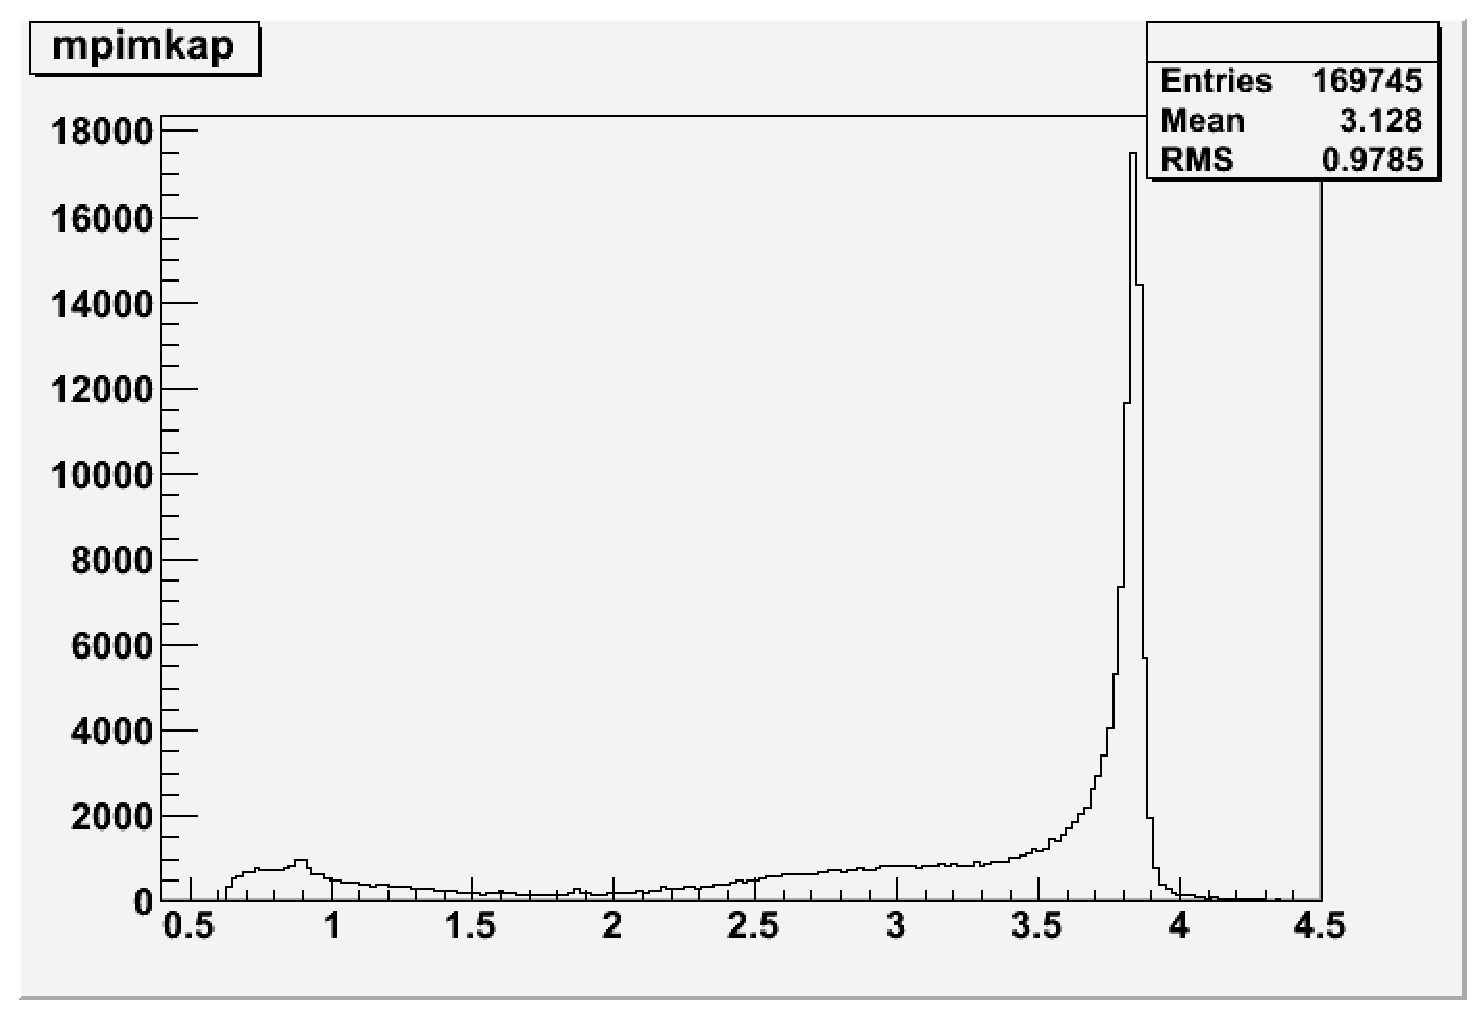
\includegraphics[width=0.4\textwidth]{Kapi/data_1.eps}}
\label{fig1.}
\caption{Distribution of $m_{K^+ \pi^-}$ from 0.4 to 4.5}
\subfigure[]{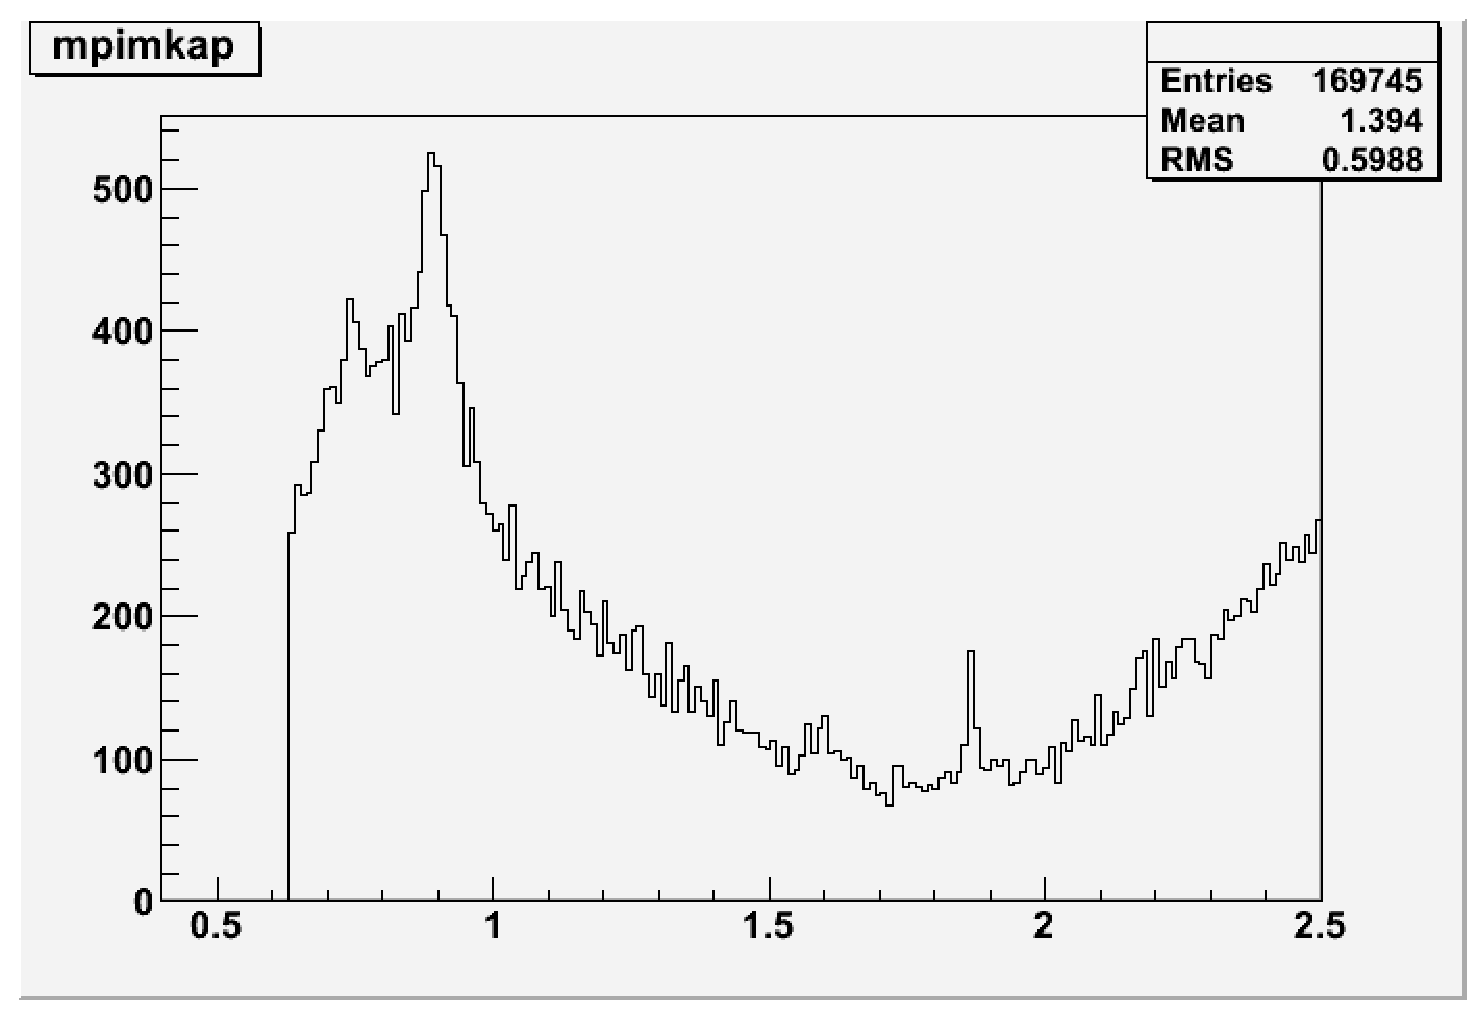
\includegraphics[width=0.4\textwidth]{Kapi/data_2.eps}}
\label{fig2.}
\caption{Distribution of $m_{K^+ \pi^-}$ from 0.4 to 2.5}
\subfigure[]{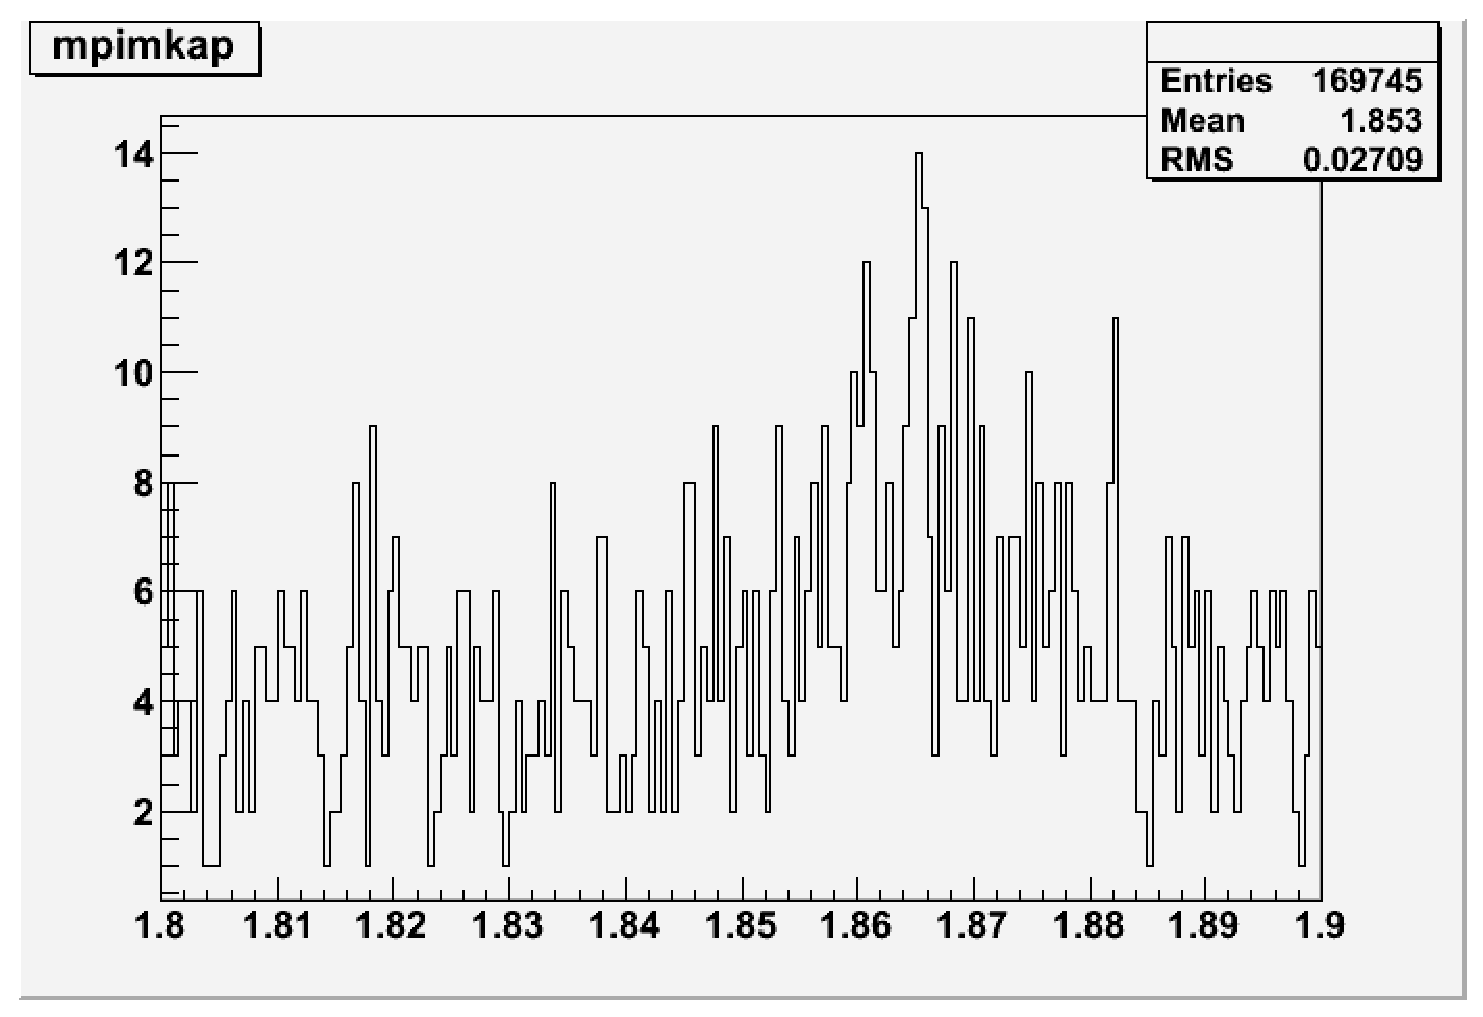
\includegraphics[width=0.4\textwidth]{Kapi/data_3.eps}}
\label{fig3.}
\caption{Distribution of $m_{K^+ \pi^-}$ from 1.8 to 1.9}
\end{figure*}
\end{frame}

\begin{frame}{The Raw Results of inclusive MC Been Acquired}
\end{frame}
\end{document}
